The Tresca or maximum shear stress yield criterion is taken to be the work of Henri Tresca. It is also referred as the Tresca-Guest (TG) criterion. The functional form of this yield criterion is
\[
f(\sigma_1,\sigma_2,\sigma_3) = 0
\]
In terms of the principal stresses the Tresca criterion is expressed as
\[
{\max(|\sigma_1 - \sigma_2| , |\sigma_2 - \sigma_3| , |\sigma_3 - \sigma_1| ) = c }
\]
The following figure shows the Tresca-Guest yield surface in the three-dimensional space of principal stresses. 
\begin{center}
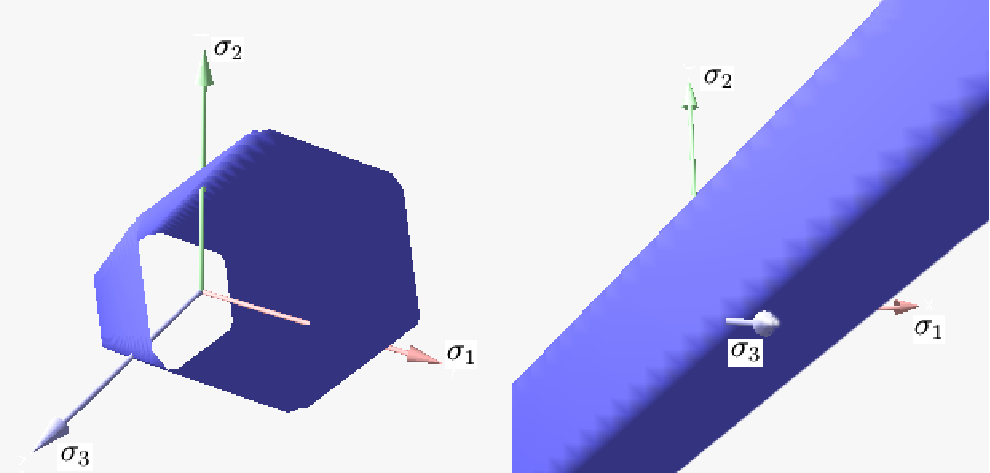
\includegraphics[width=0.6\textwidth]{images/rheology/tresca/Tresca.pdf}
\end{center}
It is a prism of six sides and having infinite length. This means that the material remains viscous when all three principal stresses are roughly equivalent (a hydrostatic pressure), no matter how much it is compressed or stretched. However, when one of principal stresses becomes smaller (or larger) than the others the material is subject to shearing. In such situations, if the shear stress reaches the yield limit then the material enters the plastic domain. 

\begin{remark}
The yield function presents sharp corners, making its numerical implementation more difficult (directional derivatives are needed)
\end{remark}


We have already established in Eq.~\ref{eq:sig13a}:
\begin{eqnarray}
\sigma_1 - \sigma_3  &=& 2 \sqrt{{\cal I}_2({\bm \tau})} \cos \theta \nn
\end{eqnarray}
with $\sigma_1>\sigma_2>\sigma_3$,
so that the failure criterion is given by
\begin{mdframed}[backgroundcolor=blue!5]
\[
F^{\text{\tiny TR}}=2\sqrt{ {\cal I}_2({\bm \tau})  } \cos \theta - c 
\]
\end{mdframed}

\Literature: \cite{long03}


%DO NOT READ FURTHER - 9dec2019
%%%%%%%%%%%%%%%%%%%%%%%%%%%%%%%%%%
%Using the values of the principal stresses in a two dimensional space, the criterion becomes 
%\[
%|\sigma_1 - \sigma_2| =\sqrt{J_2'}  = \sigma_0 
%\]
%which is equivalent to the von Mises criterion.


\newpage
